\documentclass{beamer}
%\documentclass[handout]{beamer}
\setbeamertemplate{navigation symbols}{}

\mode<presentation>
{
  \usetheme{default}
  \useinnertheme{circles}
  %\usetheme{plain}
  %  \usetheme{default}
  % or ...
  % makes uncovered text transparent
  %\setbeamercovered{transparent}
  % or whatever (possibly just delete it)
  \setbeamertemplate{frametitle}
  { 
    \begin{centering}
     \color{blue}
     %\textbf
     {\insertframetitle}
     %\texttt{\insertframetitle}
     \par
    \end{centering}
  }
}

\usepackage[english]{babel}
\usepackage[latin1]{inputenc}
\usepackage{times}
\usepackage{hyperref}
\usepackage[T1]{fontenc}
\usepackage{amsfonts,amssymb,amsmath,alltt,psfrag,stmaryrd}
\usepackage{alltt}
% newcommands etc
\renewcommand{\ttdefault}{cmtt}
\newenvironment{ttbox}{\begin{alltt}\ttbraces\small\tt}%
                      {\end{alltt}}
%the new definition of \. suppresses line breaks
\def\ttbraces{\let\.=\nobreak\chardef\{=`\{\chardef\}=`\}\chardef\|=`\\}
% used here
\newcommand{\symb}[1]{\makebox{\it #1}} 
\newcommand\dist{\ensuremath{\to_\|}}
\newcommand\ttevalsto{\mbox{\( \evalsto\ \)}}

\title[] % (optional, use only with long paper titles)
{BSc Computer Science -- First Year
}

\author[First Year Team] % (optional, use only with lots of authors)
{Tony Clark\\
Ed Currie\\
Bob Fields\\
Florian Kammueller\\
Martin Loomes\\
Rui Loureiro\\
Ralph Moseley\\
Franco Raimondi
}



\institute[University of Middlesex] % (optional, but mostly needed)
{\inst{}%
  Middlesex University London\\[2ex]
{
\includegraphics[height=1cm]{Middlesex_University_logo.png}}
}
\date[October 2013]% (optional, should be abbreviation of conference name)
{{\footnotesize 1. October 2013}}

\begin{document}

\begin{frame}
  \titlepage
\end{frame}


\setbeamertemplate{footline}{
  \begin{beamercolorbox}[wd=0.5\paperwidth,ht=0.5ex,dp=2ex,left]{date
      in head/foot}
    \hspace*{1mm}\insertframenumber
  \end{beamercolorbox}
}





\begin{frame}
\frametitle{Welcome to the Computer Science First Year}
\begin{itemize}
\item Key Aims of First Year
\item How To study it
\item LaTeX Challenge 
\item Prices
\end{itemize}
\end{frame}


\begin{frame}
\frametitle{Overview}
 \tableofcontents
\end{frame}

\section{A Typical Week}

%% Delete this, if you do not want the table of contents to pop up at
%% the beginning of each subsection:
\AtBeginSection[]
{
  \begin{frame}<beamer>
    \frametitle{Overview}
    \tableofcontents[currentsection]
  \end{frame}
}

\begin{frame}
\frametitle{Purpose of the Year}
There is one simple question we must address:
\begin{quote}
{\it Is attendance at sessions compulsory?}
\end{quote}
%
The answer is simple:
\begin{quote}
{\it No, you are perfectly free to fail if you want to.}
\end{quote}
%
\begin{figure}[t]
\centering
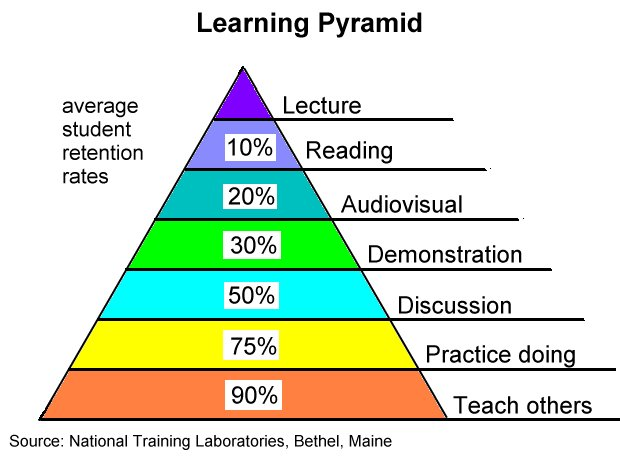
\includegraphics[width=0.6\columnwidth]{learning_pyramid}
\caption{The Learning Pyramid}
\end{figure}
\end{frame}

\section{How To Study the First Year}


\section{The LaTeX Challenge}

\begin{frame}
\frametitle{Overview of First Week}
\begin{itemize}
\item \alert{Mo 1.10.} Introduction: Martin Loomes Overview
\item Goal of the Week: LaTeX challenge

\alert{\it Produce a Latex documentation of Middlesex University}

\item \alert{Tu 2.10.} Set up:
\begin{itemize}
\item This lecture (Intro to CS program \& LaTeX chalLenge)  
\item Break out into two hour sessions in 3 or 4 groups of 30 (H10X labs)
\begin{enumerate}
\item Group formation of student teams (3 students)
\item Learn LaTeX basics
\item Start project brainstorming
\end{enumerate}
\end{itemize}
\item \alert{We 3.10, Th 4.10.} Material/Support/Equipment:
\begin{itemize}
\item Groups work on Tuesday, Wednesday, Thursday 
\item LaTeX clinic on Wednesday \& Thursday 10-15pm in H10X
\end{itemize}
\item \alert{Fr 5.10.} Presentation of best solutions and Prices
\end{itemize}
\end{frame}

\begin{frame}
\frametitle{LaTeX Challenge: Topic}
\begin{itemize}
\item Subject is Middlesex University
\item Anything goes!
\item Examples: 
\begin{itemize}
\item The university crest: history and changes
\item Where are the best coffee places?
\item How does the university work? Use a state machine to model it.
\item Student unions and sports.
\end{itemize}
\end{itemize}
\end{frame}


\begin{frame}
\frametitle{LaTeX Challenge: How To?}
\begin{itemize}
\item LaTeX: \url{http://www.latex-project.org}
\item In PC equipped Labs we will use: MikTeX \url{http://miktex.org}
\item In Mac equipped Labs we will use: Mactex 
\item Examples material is available at: 
\url{https://github.com/MiddlesexCS/latex_intro} \\
\alert{$\Rightarrow$} This talk is written in LaTeX
  and is available amongst other examples in the github (as \texttt{CS\_induction\_talk.tex})
\end{itemize}
\end{frame}

\begin{frame}
\frametitle{LaTeX Challenge: Prices}
\begin{itemize}
\item \alert{Th 4.10. 15pm} Each group of 30 decides on two top teams
\item \alert{Fr 5.10} LaTeX challenge Finals
\item Presentation of 6 Projects
\item Student Panel ranks the 6 Finalist Projects: criteria \alert{$3\times 10 = 30 points$}
\begin{itemize}
\item Technical: Use of LaTeX
\item Originality: idea, quality of content and research
\item Delivery: quality of presentation
\end{itemize}
\item Awards for Winners
\item \alert{Prices}
\begin{itemize}
\item<1-3> Of all 6 teams each member receives a Middlesex print/copy card (value 10 pounds)
\item<2-3> Runner up team members receive each a Middlesex baseball cap in addition (10 pounds each)
\item<3> Champion team members receives a Middlesex Hoodie in addition (25 pounds each)
\end{itemize}
\item<3> Overall price money: 285 pounds
\end{itemize}
\end{frame}



\end{document}

